\documentclass[10pt]{article}
\usepackage[usenames]{color} %used for font color
\usepackage{amssymb} %maths
\usepackage{amsmath} %maths
\usepackage[utf8]{inputenc} %useful to type directly diacritic characters
\usepackage[letterpaper, portrait, margin=1in]{geometry}
\usepackage{graphicx,wrapfig}
\begin{document}
\subsection*{MSDS610 Week 8 Spark Continued Assignment - Nathan Worsham}
I was very interested in this weeks assignment as it pertains to what I already work in - IT Security. I started by getting the download link and getting the data.
\begin{figure}[!h]
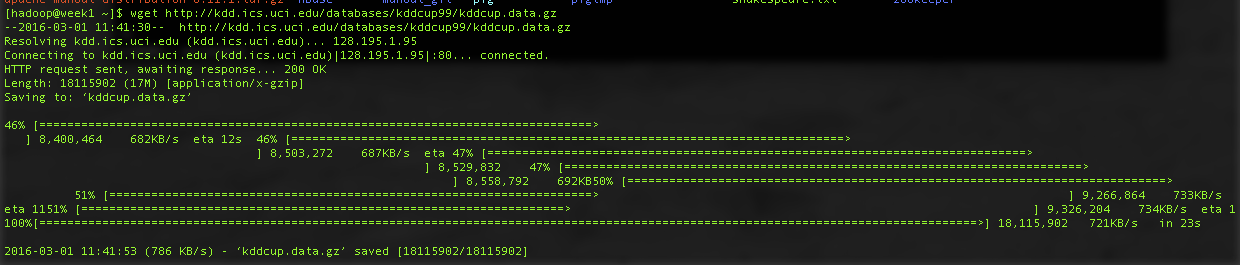
\includegraphics[scale=0.37]{wget.png}
\centering
\end{figure}\\
\indent When I tried to unpack it I received errors that \verb|tar: This does not look like a tar archive|, I had even tried providing the \verb|z| option but received the same problem and tried redownloading the file incase it was corrupted. After looking at a superuser.com (2014) question, I realized that the file likely is just a Gzip file and not a TAR. So I then used gzip to unpack it. 
\begin{figure}[!h]
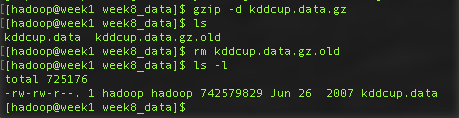
\includegraphics[scale=0.37]{gzip.png}
\centering
\end{figure}\\
\indent I went ahead and created a new folder in the HDFS and then copied the kdd data to it.
\begin{figure}[!h]
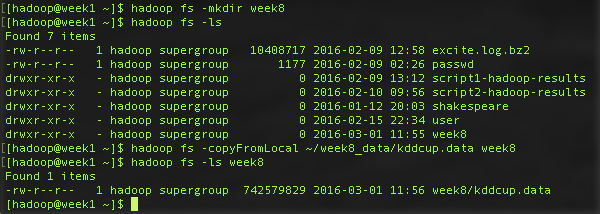
\includegraphics[scale=0.37]{copyfromlocal.png}
\centering
\end{figure}\\
\indent The spark shell is opened and the csv file is loaded as an RDD.
\begin{figure}[!h]
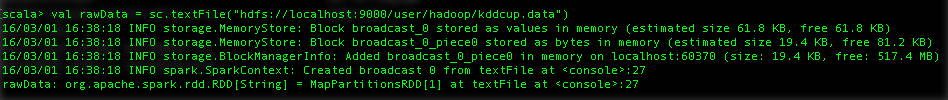
\includegraphics[scale=0.37]{RDD.png}
\centering
\end{figure}\\
\indent  I stumbled a bit on the location for the CSV file as I didn't realize the \verb|hadoop fs| command starts off in the user's home directory similar to Linux as the command kept telling me it could not find the file. Once I realized the full path was \verb|/user/hadoop/| I moved the file in the HDFS and then was able to run the command to see what labels where in the data.
\pagebreak
\begin{figure}[!h]
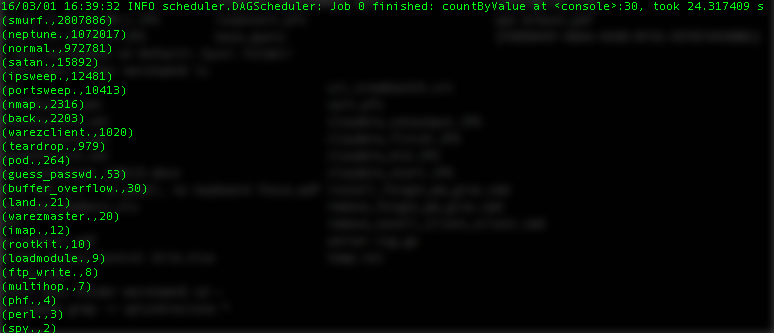
\includegraphics[scale=0.37]{labels.png}
\centering
\end{figure}\\
\indent Next the categorical values are removed as K-means clustering requires numerical data.
\begin{figure}[!h]
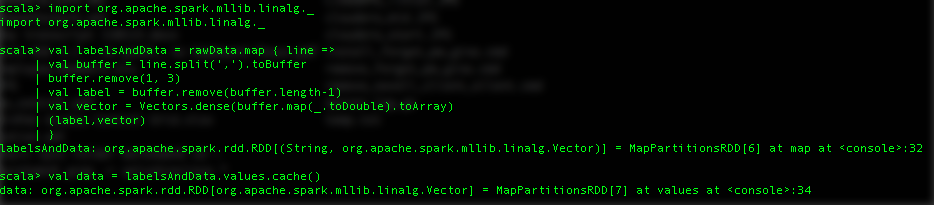
\includegraphics[scale=0.37]{removeLabels.png}
\centering
\end{figure}\\
\indent The Kmeans implementation is imported and then run on the "data" which took some time to run. Then the centroids are printed.
\begin{figure}[!h]
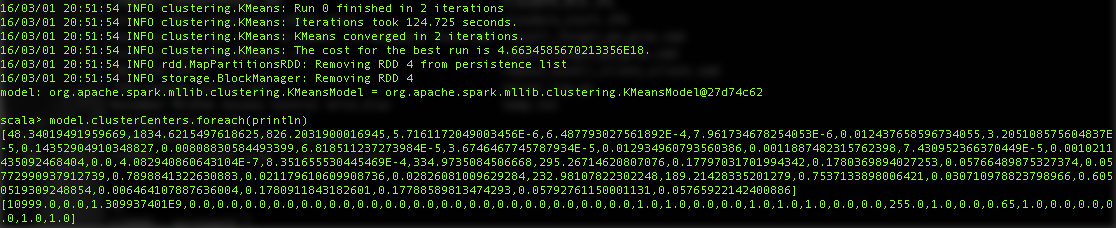
\includegraphics[scale=0.37]{printCentroids.png}
\centering
\end{figure}\\
\indent The previous model only did a fitting of 2 clusters on the data. So seeing how the existing labels lands in each cluster, all land in one cluster except for 1 "portsweep" which is a poor model then.
\par
\raisebox{-.6\height}{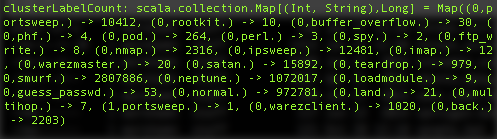
\includegraphics[width=8cm]{clusterLabelCount1.png}}%
\hfill
\raisebox{-.6\height}{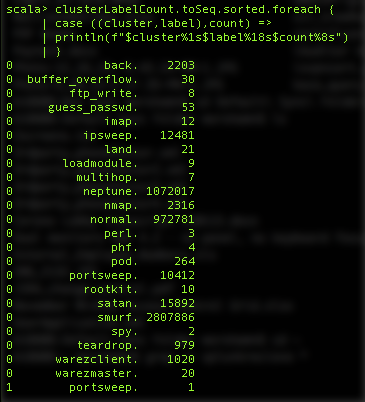
\includegraphics[width=8cm]{clusterLabelCount2.png}}%
\par
Create a function to define a Euclidean distance and another to return the distance for the data point to its cluster's centroid. This will help determine the number of clusters to use.
\begin{figure}[!h]
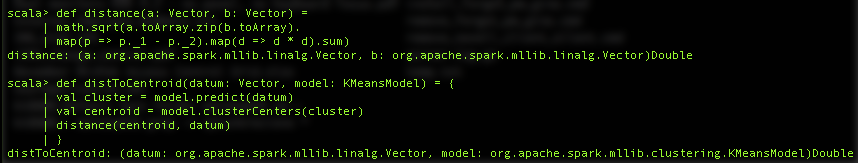
\includegraphics[scale=0.37]{2functions.png}
\centering
\end{figure}\\
\indent Now another function is created to measure the average distance from the data points to the centroids.
\begin{figure}[!h]
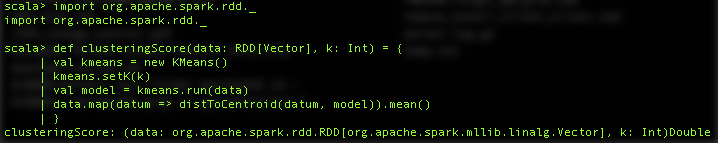
\includegraphics[scale=0.37]{avgDist.png}
\centering
\end{figure}\\
\indent Now use this function to evaluate values of k from 5 to 40, counting by 5s. Like the example, the value actually increases for 35, though they received a better output for 30 than I did. 
\begin{figure}[!h]
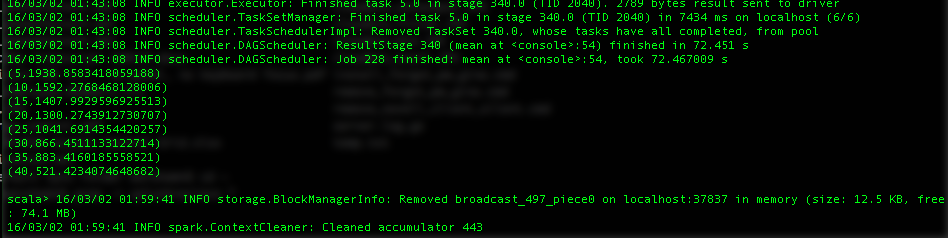
\includegraphics[scale=0.37]{evaluateK.png}
\centering
\end{figure}\\
\indent Running the iteration longer and decrease the threshold for the minimum amount considered significant and then finally run in parallel with \verb|par.map|. Took longer to run than the previous but in my results the output starts to increase at 100 with 90 being the best.
\par
\raisebox{-.6\height}{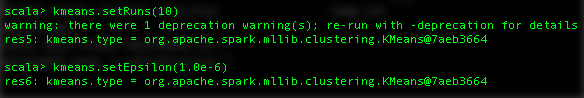
\includegraphics[width=8cm]{epsillion.png}}%
\hfill
\raisebox{-.6\height}{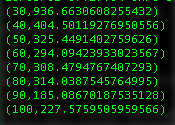
\includegraphics[width=8cm]{evaluateK2.png}}%
\par
Changing each feature into a Z-score or standard score can help normalize the output. This is done by subtracting the mean and dividing by the standard deviation. Various outputs leading up to the final output.\\
n
\begin{figure}[!h]
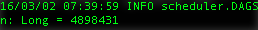
\includegraphics[scale=0.43]{n.png}
\centering
\end{figure}\\
\pagebreak
sums
\begin{figure}[!h]
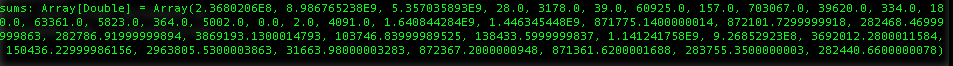
\includegraphics[scale=0.37]{sum.png}
\centering
\end{figure}\\
sum-of-squares
\begin{figure}[!h]
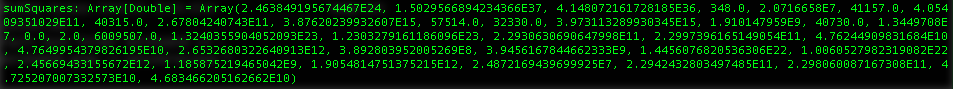
\includegraphics[scale=0.37]{sumSquares.png}
\centering
\end{figure}\\
standard deviation and means
\begin{figure}[!h]
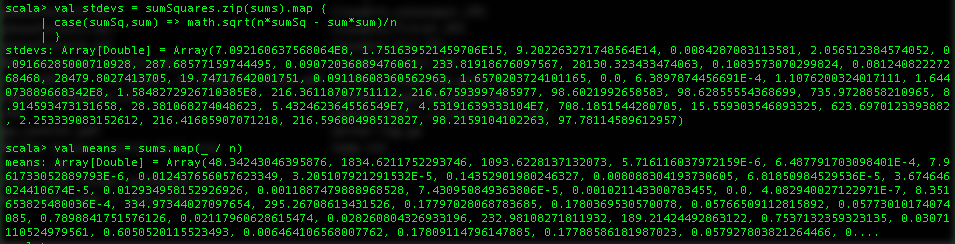
\includegraphics[scale=0.37]{stDev_and_means.png}
\centering
\end{figure}\\
normalize function
\begin{figure}[!h]
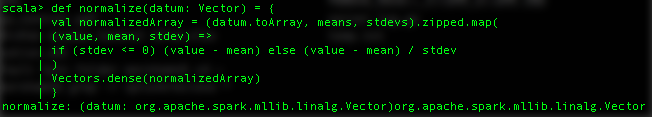
\includegraphics[scale=0.37]{normalizeFunction.png}
\centering
\end{figure}\\
\indent Finally the output of the k values using standard score, this time my output was similar to the example as 100 seems to be the good spot from this data.
\begin{figure}[!h]
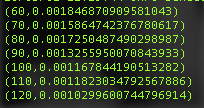
\includegraphics[scale=0.37]{standardScore.png}
\centering
\end{figure}\\
\indent Using "one-hot" encoding, the categorical values are brought back in as features for consideration in the k-means clustering. I used the code they offered from git, but I have to say the code versus the book is not exactly one-to-one and can be confusing finding where they meet up. My output was a bit different from theirs as mine is much bigger values and 160 has the lowest value, which might be explained by using the code from git. Unfortunately it took much too long to get those results that I was not going to try running it again. 
\begin{figure}[!h]
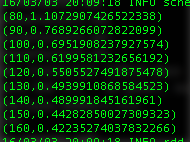
\includegraphics[scale=0.37]{oneHotCategory.png}
\centering
\end{figure}\\
\indent Worrying about how long the last clustering portion took, I wanted to just use their recommendation of k=150 and move onto the end, in order to make sure I could complete the assignment on time. 
\pagebreak
\begin{figure}[!h]
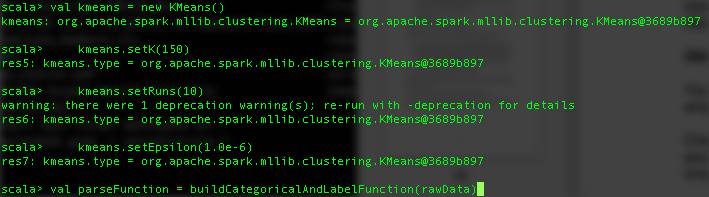
\includegraphics[scale=0.37]{k150.png}
\centering
\end{figure}\\
\indent Again I was trying my best at following along with their code from git, but this time I was resolved to run it in pieces if I could. I also shutdown my VM and gave it another cpu and another GB of RAM to try to help the number crunching and time to complete.
\begin{figure}[!h]
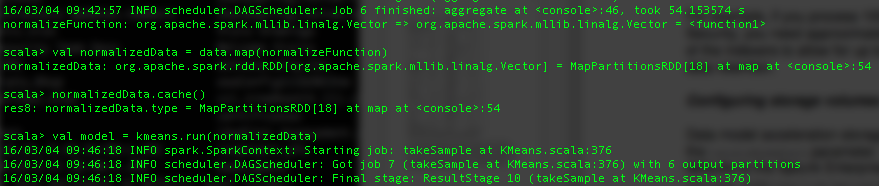
\includegraphics[scale=0.37]{buildNewModel.png}
\centering
\end{figure}\\
\indent But as it turns out the only portion that took time to compute was the \verb|val model = kmeans.run(normalizedData|). As expected there are many more centroids now.
\begin{figure}[!h]
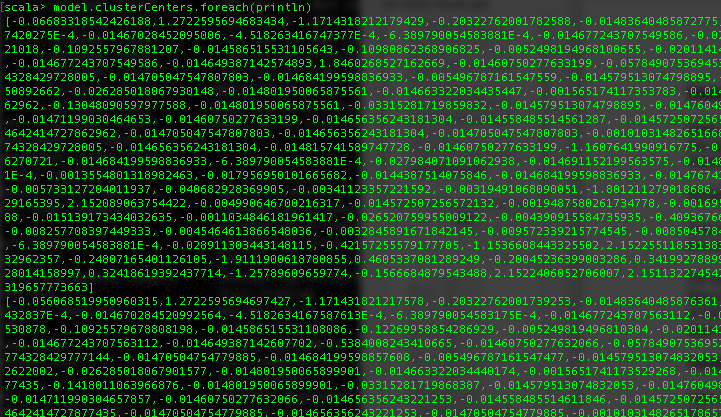
\includegraphics[scale=0.37]{newCentroids.png}
\centering
\end{figure}\\
\indent After that I went ahead and tried printing the clusters with labels as before like the book showed using their val \verb|clusterLabelCount| but I received several errors and a driver stacktrace that I wasn't sure about so I moved onto the anomaly detection. Here in the git code the line 
\begin{verbatim}
val anomalyDetector = buildAnomalyDetector(data, normalizeFunction)
\end{verbatim}
calls the entire previous function, so I ran the rest of that function and then assumed that the value \verb|anomolyDetector| needed to equal the output of the function \verb|buildAnomalyDetector|.
\begin{figure}[!h]
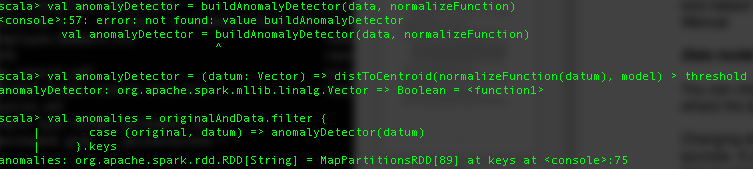
\includegraphics[scale=0.37]{functionOutput.png}
\centering
\end{figure}\\
\indent But then I realized the book's code spells this out differently than the git code and takes this into account. 
\pagebreak
\begin{figure}[!h]
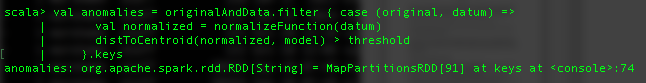
\includegraphics[scale=0.37]{bookFunction.png}
\centering
\end{figure}\\
\indent Either way they both end up with the same output on anomalies.
\begin{figure}[!h]
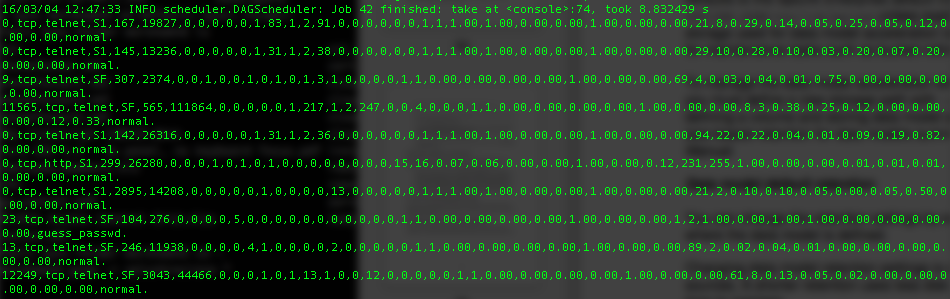
\includegraphics[scale=0.37]{finalOutput.png}
\centering
\end{figure}\\
\indent The most anomalous event the book had was contained in my top 10 output, but is the 6th listing. My first listing is a telnet connection. I was curious about the connections--more specifically my top listing, so I went back to the KDD cup data for what the columns represented. Also using this site--ita.ee.lbl.gov(Paxson, nd) to understand the "flags". It would seem that an "S1" state is for when 2 sides have established a connection (TCP handshake) but nothing further has been "seen". Though according to the listing, the destination has received 19827 bytes. Telnet connections nowadays themselves are anomalous if they are seen over the internet because they are not a secure connection--anyone listening could see exactly what transpired, in 1999 that probably would have been common to see but today it is replaced by SSH and other more secure communication methods. My guess would be that the connection is anomalous because there are multiple 100\% error rates (3x) happening on this connection.\\
\indent When I had shutdown my VM to give it more resources I also exported a copy of it. While I was running the computations for the anomaly detector I started up the cloned VM on another computer and ran the clustering take-4 functions from the git code--the labels with entropy. This time I ended up receiving a similar output to the book that pointed to k=150 was a good choice.
\par
\raisebox{-.6\height}{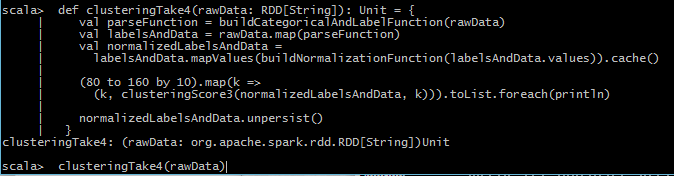
\includegraphics[width=9cm]{clusteringTake4.png}}%
\hfill
\raisebox{-.6\height}{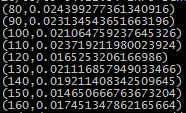
\includegraphics[width=7cm]{entropy.png}}%
\par
\subsection*{References}
superuser.com, 2014. Retrieved from http://superuser.com/questions/841865/extracting-a-tar-gz-file-returns-this-does-not-look-like-a-tar-archive\\
UCI KDD Archive, 1999. Retrieved from http://kdd.ics.uci.edu/databases/kddcup99/kddcup99.html\\
Paxson, Vern. n.d. Retrieved from http://ita.ee.lbl.gov/html/contrib/tcp-reduce-doc.html
\end{document}
